\documentclass[aspectratio=169,11pt]{beamer}

\makeatletter
\NeedsTeXFormat{LaTeX2e}
\ProvidesPackage{beamerthemeDUNEProfessional}[2026/08/19 DUNE professional Beamer theme]

\mode<presentation>

\RequirePackage{iftex}
\RequirePackage{graphicx}
\RequirePackage{xcolor}
\RequirePackage{tikz}
\RequirePackage{adjustbox}
\RequirePackage{array}
\RequirePackage{booktabs}
\RequirePackage{tabularx}
\RequirePackage{ragged2e}

\usetikzlibrary{arrows.meta,calc,fit,positioning,shapes.geometric}

\useinnertheme{default}
\useoutertheme{default}
\usefonttheme{professionalfonts}
\setbeamertemplate{navigation symbols}{}

% Logo path is relative to a deck directory. Override with \DuneSetLogoPath.
\newcommand{\DuneLogoPath}{../../templates/dune-professional/logos}
\newcommand{\DuneSetLogoPath}[1]{\renewcommand{\DuneLogoPath}{#1}}

% Color roles. Keep semantic names in decks; avoid ad hoc local colors.
\definecolor{DuneBg}{HTML}{101820}
\definecolor{DunePanel}{HTML}{1B2733}
\definecolor{DunePanelAlt}{HTML}{263645}
\definecolor{DuneTitleBand}{HTML}{20303E}
\definecolor{DuneLine}{HTML}{536878}
\definecolor{DuneText}{HTML}{F1F5F7}
\definecolor{DuneMuted}{HTML}{BAC6CF}
\definecolor{DuneOrange}{HTML}{F2682B}
\definecolor{DuneCyan}{HTML}{8EDDF2}
\definecolor{DuneMint}{HTML}{9BD7AE}
\definecolor{DuneYellow}{HTML}{E8C85A}
\definecolor{DuneRed}{HTML}{F38B7F}
\definecolor{DuneViolet}{HTML}{B8A7E8}

\setbeamercolor{normal text}{fg=DuneText,bg=DuneBg}
\setbeamercolor{title}{fg=white,bg=DuneBg}
\setbeamercolor{subtitle}{fg=DuneMuted,bg=DuneBg}
\setbeamercolor{author}{fg=DuneCyan,bg=DuneBg}
\setbeamercolor{date}{fg=DuneMuted,bg=DuneBg}
\setbeamercolor{frametitle}{fg=white,bg=DuneBg}
\setbeamercolor{headline}{fg=DuneMuted,bg=DuneBg}
\setbeamercolor{footline}{fg=DuneMuted,bg=DuneBg}
\setbeamercolor{itemize item}{fg=DuneOrange}
\setbeamercolor{itemize subitem}{fg=DuneCyan}
\setbeamercolor{enumerate item}{fg=DuneOrange}
\setbeamercolor{caption name}{fg=DuneMuted}

\setbeamercolor{dune panel}{fg=DuneText,bg=DunePanel}
\setbeamercolor{dune panel alt}{fg=DuneText,bg=DunePanelAlt}
\setbeamercolor{dune accent}{fg=DuneBg,bg=DuneCyan}
\setbeamercolor{dune decision}{fg=DuneBg,bg=DuneYellow}
\setbeamercolor{dune risk}{fg=DuneBg,bg=DuneRed}
\setbeamercolor{dune evidence}{fg=DuneBg,bg=DuneMint}
\setbeamercolor{dune violet}{fg=DuneBg,bg=DuneViolet}

\setbeamerfont{normal text}{size=\small}
\setbeamerfont{title}{series=\bfseries}
\setbeamerfont{subtitle}{size=\large}
\setbeamerfont{author}{size=\normalsize,series=\bfseries}
\setbeamerfont{date}{size=\small}
\setbeamerfont{frametitle}{series=\bfseries}
\setbeamerfont{footline}{size=\scriptsize}

\ifPDFTeX
  \RequirePackage[scaled]{helvet}
  \renewcommand*\familydefault{\sfdefault}
  \RequirePackage[T1]{fontenc}
\else
  \RequirePackage{fontspec}
  \defaultfontfeatures{Ligatures=TeX,Scale=MatchLowercase}
  \IfFontExistsTF{IBM Plex Sans}{
    \setsansfont{IBM Plex Sans}
    \setmainfont{IBM Plex Sans}
  }{
    \IfFontExistsTF{Helvetica Neue}{
      \setsansfont{Helvetica Neue}
      \setmainfont{Helvetica Neue}
    }{
      \IfFontExistsTF{TeX Gyre Heros}{
        \setsansfont{TeX Gyre Heros}
        \setmainfont{TeX Gyre Heros}
      }{
        \IfFontExistsTF{Liberation Sans}{
          \setsansfont{Liberation Sans}
          \setmainfont{Liberation Sans}
        }{
          \setsansfont{DejaVu Sans}
          \setmainfont{DejaVu Sans}
        }
      }
    }
  }
  \IfFontExistsTF{JetBrains Mono}{
    \setmonofont{JetBrains Mono}[Scale=0.88]
  }{
    \IfFontExistsTF{Latin Modern Mono}{
      \setmonofont{Latin Modern Mono}[Scale=0.88]
    }{
      \setmonofont{DejaVu Sans Mono}[Scale=0.88]
    }
  }
  \renewcommand*\familydefault{\sfdefault}
\fi

\setbeamersize{text margin left=0.78cm,text margin right=0.78cm}
\setlength{\leftmargini}{1.15em}
\setlength{\leftmarginii}{1.05em}
\setlength{\parskip}{0.18em}

\setbeamertemplate{itemize item}{%
  \color{DuneOrange}\raisebox{0.15ex}{\scriptsize$\blacktriangleright$}%
}
\setbeamertemplate{itemize subitem}{%
  \color{DuneCyan}\raisebox{0.15ex}{\tiny$\blacktriangleright$}%
}

% Measured boxes: content may shrink down, but never expands outside the safe box.
\newcommand{\DuneFitBox}[3]{%
  \begin{adjustbox}{max width=#1,max totalheight=#2}%
    \begin{minipage}{#1}\raggedright #3\end{minipage}%
  \end{adjustbox}%
}

\newcommand{\DuneTightList}{%
  \setlength{\itemsep}{0.45mm}%
  \setlength{\parskip}{0pt}%
}

\newcommand{\DuneEyebrow}[1]{%
  {\color{DuneCyan}\scriptsize\bfseries #1\par}%
}

\newcommand{\DunePill}[2]{%
  \tikz[baseline=-0.55ex]\node[
    rounded corners=2.5pt,
    draw=#1,
    fill=#1!18!DuneBg,
    inner xsep=4pt,
    inner ysep=1.35pt,
    text=#1,
    font=\tiny\bfseries
  ]{#2};%
}

\newcommand{\DuneCard}[4][dune panel]{%
  \begin{beamercolorbox}[wd=\linewidth,sep=5pt,rounded=true]{#1}
    {\usebeamercolor[fg]{#1}\bfseries #2\par}
    \vspace{0.4mm}
    {\usebeamercolor[fg]{#1}\footnotesize #3\par}
    \if\relax\detokenize{#4}\relax\else
      \vspace{0.5mm}{\usebeamercolor[fg]{#1}\scriptsize #4\par}
    \fi
  \end{beamercolorbox}
}

\newcommand{\DuneFixedCard}[5][dune panel]{%
  \begin{beamercolorbox}[wd=\linewidth,sep=5pt,rounded=true]{#1}
    \begin{minipage}[t][#2][t]{\dimexpr\linewidth-10pt\relax}
      \raggedright
      {\usebeamercolor[fg]{#1}\bfseries #3\par}
      \vspace{0.45mm}
      {\usebeamercolor[fg]{#1}\footnotesize #4\par}
      \if\relax\detokenize{#5}\relax\else
        \vspace{0.55mm}{\usebeamercolor[fg]{#1}\scriptsize #5\par}
      \fi
    \end{minipage}
  \end{beamercolorbox}
}

\newcommand{\DuneFooterLogo}{%
  \IfFileExists{\DuneLogoPath/logosolo.png}{%
    \tikz[baseline=-0.52ex]\node[opacity=0.42,inner sep=0pt]{%
      \includegraphics[height=0.25cm]{\DuneLogoPath/logosolo.png}%
    };%
  }{}%
}

\newcommand{\DuneTalkDate}{%
  \@ifundefined{mydate}{\today}{\mydate}%
}

% Background and fixed frame-title band.
\addtobeamertemplate{background canvas}{%
  \begin{tikzpicture}[remember picture,overlay]
    \fill[DuneBg] (current page.south west) rectangle (current page.north east);
    \draw[DuneLine,line width=0.55pt]
      ($(current page.south west)+(0.78,0.74)$)
      -- ($(current page.south east)+(-0.78,0.74)$);
    \fill[DuneCyan!16]
      ($(current page.south east)+(-3.2,0.83)$) rectangle ++(1.45,0.055);
  \end{tikzpicture}%
}{}

\setbeamertemplate{headline}{}

\setbeamertemplate{frametitle}{%
  \nointerlineskip%
  \begin{tikzpicture}[remember picture,overlay]
    \fill[DuneTitleBand]
      (current page.north west) rectangle ($(current page.north east)+(0,-1.18)$);
    \fill[DuneOrange]
      ($(current page.north west)+(0.78,-0.23)$) rectangle ++(1.38,0.055);
    \node[anchor=west,inner sep=0pt]
      at ($(current page.north west)+(0.78,-0.72)$) {%
        \DuneFitBox{\dimexpr\paperwidth-1.56cm\relax}{6.7mm}{%
          {\color{white}\bfseries\fontsize{17}{20}\selectfont\insertframetitle}%
        }%
      };
    \ifx\insertframesubtitle\@empty\else
      \node[anchor=west,inner sep=0pt]
        at ($(current page.north west)+(0.78,-1.02)$) {%
          \DuneFitBox{\dimexpr\paperwidth-1.56cm\relax}{3.2mm}{%
            {\color{DuneMuted}\scriptsize\insertframesubtitle}%
          }%
        };
    \fi
  \end{tikzpicture}%
  \vspace*{12.5mm}%
}

\setbeamertemplate{footline}{%
  \leavevmode%
  \begin{beamercolorbox}[wd=\paperwidth,ht=6.4mm,dp=1.8mm,leftskip=0.78cm,rightskip=0.78cm]{footline}
    \DuneFooterLogo\hspace{0.45em}{\textcolor{DuneMuted}{\DuneTalkDate}}%
    \hfill%
    {\textcolor{DuneOrange}{\bfseries\insertframenumber}\textcolor{DuneMuted}{/\inserttotalframenumber}}%
  \end{beamercolorbox}%
}

\setbeamertemplate{title page}{%
  \begin{tikzpicture}[remember picture,overlay]
    \fill[DuneBg] (current page.south west) rectangle (current page.north east);
    \fill[DuneTitleBand]
      (current page.north west) rectangle ($(current page.north east)+(0,-3.03)$);
    \fill[DuneOrange]
      ($(current page.north west)+(0.82,-0.58)$) rectangle ++(1.55,0.075);
    \fill[DuneCyan]
      ($(current page.south east)+(-2.8,0.79)$) rectangle ++(1.88,0.065);
    \IfFileExists{\DuneLogoPath/DUNElogo_white.png}{%
      \node[anchor=south east,opacity=0.13,inner sep=0pt]
        at ($(current page.south east)+(-0.55,1.42)$) {%
        \includegraphics[width=0.34\paperwidth]{\DuneLogoPath/DUNElogo_white.png}%
      };
    }{}%
    \IfFileExists{\DuneLogoPath/FNAL-Logo-NAL-Light.png}{%
      \node[anchor=south east,inner sep=0pt]
        at ($(current page.south east)+(-0.92,0.78)$) {%
        \includegraphics[height=0.42cm]{\DuneLogoPath/FNAL-Logo-NAL-Light.png}%
      };
    }{}%
    \node[anchor=north west,inner sep=0pt]
      at ($(current page.north west)+(0.82,-0.88)$) {%
        \DuneFitBox{0.78\paperwidth}{1.48cm}{%
          {\color{white}\bfseries\fontsize{25}{28}\selectfont\inserttitle}%
        }%
      };
    \node[anchor=north west,inner sep=0pt]
      at ($(current page.north west)+(0.82,-3.55)$) {%
        \DuneFitBox{0.56\paperwidth}{1.35cm}{%
          {\color{DuneMuted}\fontsize{13}{17}\selectfont\insertsubtitle}%
        }%
      };
    \node[anchor=north west,text=DuneCyan,font=\bfseries,inner sep=0pt]
      at ($(current page.north west)+(0.82,-6.3)$) {\insertauthor};
    \node[anchor=north west,text=DuneMuted,font=\small,inner sep=0pt]
      at ($(current page.north west)+(0.82,-6.82)$) {\insertdate};
  \end{tikzpicture}%
  \vfill%
}

\tikzset{
  dune repo/.style={
    draw=DuneCyan,
    fill=DuneCyan!12!DunePanel,
    text=DuneText,
    rounded corners=3pt,
    align=center,
    text width=2.35cm,
    minimum height=0.86cm,
    inner sep=4pt,
    font=\scriptsize\bfseries
  },
  dune repo muted/.style={
    draw=DuneLine,
    fill=DunePanelAlt,
    text=DuneText,
    rounded corners=3pt,
    align=center,
    text width=2.35cm,
    minimum height=0.86cm,
    inner sep=4pt,
    font=\scriptsize\bfseries
  },
  dune artifact/.style={
    draw=DuneMint,
    fill=DuneMint!13!DunePanel,
    text=DuneText,
    rounded corners=3pt,
    align=center,
    text width=2.35cm,
    minimum height=0.86cm,
    inner sep=4pt,
    font=\scriptsize\bfseries
  },
  dune decision node/.style={
    draw=DuneYellow,
    fill=DuneYellow!14!DunePanel,
    text=DuneText,
    rounded corners=3pt,
    align=center,
    text width=2.35cm,
    minimum height=0.86cm,
    inner sep=4pt,
    font=\scriptsize\bfseries
  },
  dune flow/.style={-Latex,draw=DuneCyan,line width=0.85pt},
  dune relation/.style={draw=DuneMuted,line width=0.65pt},
  dune evidence flow/.style={-Latex,draw=DuneViolet,dashed,line width=0.85pt},
  dune label/.style={
    fill=DuneBg,
    text=DuneMuted,
    inner sep=1.5pt,
    font=\tiny,
    align=center
  }
}

\mode<all>

\makeatother

\title[DAPHNE at PAB]{Qualifying ten DAPHNE boards at PAB}
\subtitle{One board at a time, with four-link streaming, Iceberg timing, power measurements, and self-trigger data}
\author{Manuel Arroyave}
\date{Engineering coordination discussion -- 24 August 2026}
\newcommand{\mydate}{24 August 2026}
\hypersetup{colorlinks=true,urlcolor=DuneInfo,linkcolor=DuneInfo}

\newcommand{\ReadbackCell}[2]{%
  \RaggedRight\textbf{#1}\par{\footnotesize\color{DuneTextMuted}#2}%
}

\tikzset{
  qa node/.style={
    rounded corners=5pt,
    align=center,
    text width=2.02cm,
    minimum height=1.05cm,
    inner sep=6pt,
    font=\small\bfseries
  },
  qa ink/.style={qa node,draw=DuneBorder,fill=DuneSurfaceRaised,text=DuneText},
  qa paper/.style={qa node,draw=DunePaper,fill=DunePaper,text=DuneOnAccent},
  qa sky/.style={qa node,draw=DuneSky,fill=DuneSky,text=DuneOnAccent},
  qa coral/.style={qa node,draw=DuneCoral,fill=DuneCoral,text=DuneOnAccent},
  qa flow/.style={-Latex,draw=DuneSky,line width=1.1pt},
  qa active flow/.style={-Latex,draw=DuneCoral,line width=1.1pt}
}

\begin{document}

\begin{frame}[plain]
  \titlepage
\end{frame}

\begin{frame}{Ten boards need one stable test, not ten simultaneous slots}
  \begin{columns}[T,onlytextwidth]
    \begin{column}{0.59\textwidth}
      \DuneBigStatement{THE PROPOSAL}
        {Move the boards to PAB and qualify them sequentially on Iceberg.}
        {We install one DAPHNE, run all four of its data links together, close its evidence, and only then move to the next serial number.}
    \end{column}
    \begin{column}{0.37\textwidth}
      \DuneCompactNumberBlock{paper}{10}{Boards in the campaign}
        {Every board follows the same frozen run card.}
      \smallskip
      \DuneCompactNumberBlock{coral}{01}{Active board}
        {Power, timing, configuration, and DAQ focus on one device.}
      \smallskip
      \DuneCompactNumberBlock{sky}{04}{Simultaneous data links}
        {The active board must sustain full streaming on all four links.}
    \end{column}
  \end{columns}
\end{frame}

\begin{frame}{PAB gives us the timing and DAQ context the bench cannot}
  \begin{columns}[T,onlytextwidth]
    \begin{column}{0.55\textwidth}
      \DuneFixedColorBlock{sky}{5.0cm}{WHY ICEBERG}
        {Use the infrastructure that already exists}
        {Iceberg has the hardware needed to exercise the timing master and DUNE DAQ data-taking path together. That lets us test board behavior in the environment we actually care about.\par\medskip
         We still keep a standalone clock routine so a board can be brought up when timing is unavailable.}
    \end{column}
    \begin{column}{0.41\textwidth}
      \DuneColorBlock{paper}{WHAT MOVES}
        {A ten-board campaign}
        {Boards, approved firmware artifacts, configuration templates, cable map, and the test guide.}
      \smallskip
      \DuneColorBlock{coral}{WHAT MUST BE READY FIRST}
        {A rehearsed DAQ 5.x workarea}
        {One-board/four-link topology, timing commands, monitoring, data check, storage, and recovery.}
    \end{column}
  \end{columns}
\end{frame}

\begin{frame}{The fixture serves one active board from end to end}
  \centering
  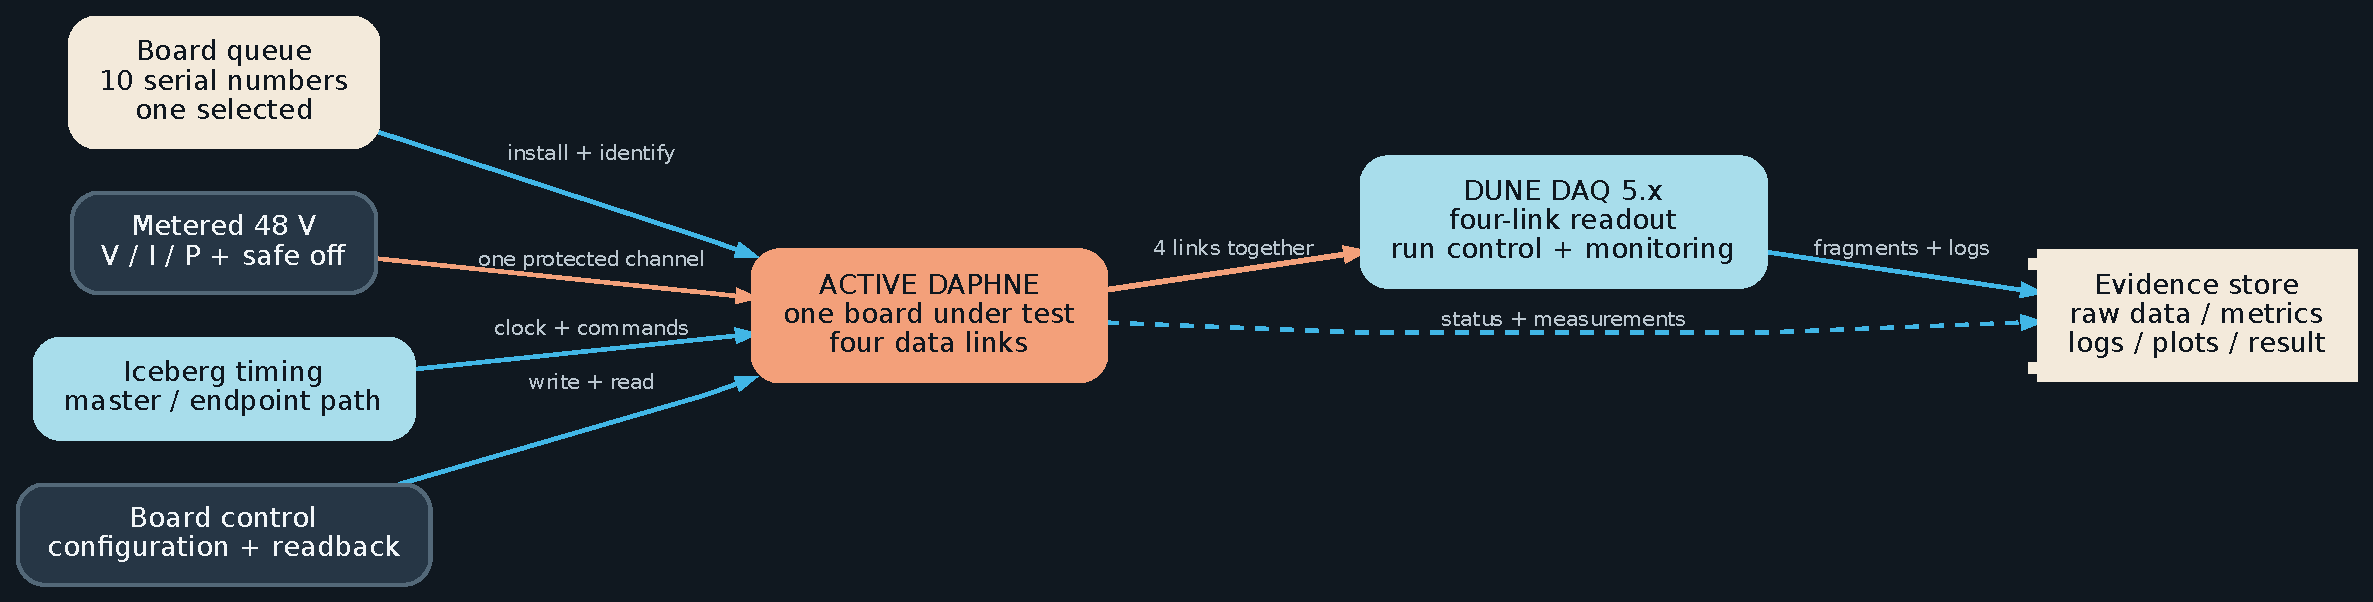
\includegraphics[width=0.97\textwidth,height=0.64\textheight,keepaspectratio]{diagrams/stand-topology.pdf}

  \smallskip
  \DuneDiagramCaption{Ten serial numbers move through one fixed fixture. The instantaneous requirement is one metered power path, one timing path, and four DAQ data links.}
\end{frame}

\DuneSectionPage{PROVE THE BASELINE FIRST}{Qualify full-stream behavior before changing firmware}
  {A known board proves the fixture; each campaign board then repeats the same configuration, timing, data, and power checks.}

\begin{frame}{The campaign advances only after four gates pass}
  \begin{columns}[T,onlytextwidth]
    \begin{column}{0.235\textwidth}
      \DuneNumberBlock{paper}{01}{Stand ready}
        {Pin DAQ 5.x, map four links, check timing, power, cooling, and storage.}
    \end{column}
    \begin{column}{0.235\textwidth}
      \DuneNumberBlock{sky}{02}{Known board}
        {Run the complete procedure and fix the fixture before the campaign.}
    \end{column}
    \begin{column}{0.235\textwidth}
      \DuneNumberBlock{sky}{03}{Full stream}
        {Four links, timing behavior, data quality, power profile, and recovery pass.}
    \end{column}
    \begin{column}{0.235\textwidth}
      \DuneNumberBlock{coral}{04}{Self-trigger}
        {Firmware update, rollback, reconfiguration, timing, and triggered data pass.}
    \end{column}
  \end{columns}

  \medskip
  \DuneCompactColorBlock{paper}{AFTER THE DRY RUN}{Freeze the fixture and run card}
    {During boards 01--10, only serial-specific identity and approved calibration/configuration values should change.}
\end{frame}

\begin{frame}{Every board begins with identity and complete readback}
  \begin{columns}[T,onlytextwidth]
    \begin{column}{0.56\textwidth}
      \footnotesize
      \renewcommand{\arraystretch}{1.00}
      \begin{tabularx}{\linewidth}{@{}p{0.30\linewidth} X@{}}
        \toprule
        Check & Save in the run directory \\
        \midrule
        Identity + firmware & \ReadbackCell{Exact board and image}{Serial, MAC/IP, fixture position, operator, image checksum, register map.} \\
        Services & \ReadbackCell{Small probes}{Ping, board service, Hermes/IPbus magic read.} \\
        Configuration & \ReadbackCell{Write, then read back}{Clock, AFE, gain, offset, threshold, mask, links, timing, sensors.} \\
        Safe baseline & \ReadbackCell{Idle point}{Links off, clocks stable, temperatures normal, metered V/I/P.} \\
        \bottomrule
      \end{tabularx}
    \end{column}
    \begin{column}{0.40\textwidth}
      \DuneCompactColorBlock{paper}{THE FIRST GATE}
        {Know exactly what is installed}
        {Serial, firmware, requested configuration, and readback must agree before streaming.}
    \end{column}
  \end{columns}
\end{frame}

\begin{frame}{Enable all four data links in controlled steps}
  \begin{columns}[T,onlytextwidth]
    \begin{column}{0.235\textwidth}
      \DuneNumberBlock{paper}{00}{Configured idle}
        {Data links disabled; record the first stable power and temperature point.}
    \end{column}
    \begin{column}{0.235\textwidth}
      \DuneNumberBlock{sky}{01}{One link}
        {Prove endpoint mapping, frame decoding, and a clean start/stop.}
    \end{column}
    \begin{column}{0.235\textwidth}
      \DuneNumberBlock{sky}{02}{Two links}
        {Check concurrency, rate, link counters, and the power increase.}
    \end{column}
    \begin{column}{0.235\textwidth}
      \DuneNumberBlock{coral}{04}{Four links}
        {Stream all four together, then hold a sustained run and repeat start/stop.}
    \end{column}
  \end{columns}

  \medskip
  \DuneCompactColorBlock{paper}{A FULL-STREAM PASS}{Data, waveforms, and operating behavior agree}
    {Check fragment and sequence continuity, malformed or dropped data, representative waveforms, per-channel baseline and RMS, timestamps, input power, and temperature.}
\end{frame}

\begin{frame}{Local timing is useful, but it is not synchronization}
  \begin{columns}[T,onlytextwidth]
    \begin{column}{0.48\textwidth}
      \DuneFixedColorBlock{paper}{3.45cm}{STANDALONE MODE}
        {Prove the board can operate locally}
        {Select the local clock. Configure and stream while reading timing status.\par\smallskip
         \textbf{Claim:} local-clock board operation works.\par
         \textbf{Not a claim:} endpoint synchronization.}
    \end{column}
    \begin{column}{0.48\textwidth}
      \DuneFixedColorBlock{sky}{3.45cm}{ICEBERG-CONNECTED MODE}
        {Prove endpoint behavior while taking data}
        {Select the endpoint source after clock and FPGA readiness. Verify both locks, address, ready state, and timestamp validity.\par\smallskip
         \textbf{Claim:} synchronization and usable timestamps remain stable.}
    \end{column}
  \end{columns}

  \smallskip
  \DuneCompactColorBlock{coral}{THE RULE}{Report the mode with every result}
    {A standalone success is a valid bring-up result, but it cannot be reported as an endpoint-timing pass.}
\end{frame}

\begin{frame}{Timing must survive commands, data-taking, and recovery}
  \begin{columns}[T,onlytextwidth]
    \begin{column}{0.235\textwidth}
      \DuneCompactNumberBlock{paper}{01}{Reach ready}
        {Select the endpoint and verify locks, address, FSM state, and valid timestamp.}
    \end{column}
    \begin{column}{0.235\textwidth}
      \DuneCompactNumberBlock{sky}{02}{Issue commands}
        {Use the timing/run-control sequence agreed by the timing and DAQ owners.}
    \end{column}
    \begin{column}{0.235\textwidth}
      \DuneCompactNumberBlock{sky}{03}{Correlate data}
        {Match command logs and state changes to run boundaries and decoded timestamps.}
    \end{column}
    \begin{column}{0.235\textwidth}
      \DuneCompactNumberBlock{coral}{04}{Recover once}
        {Use one approved reset or source transition and measure the return to ready.}
    \end{column}
  \end{columns}

  \medskip
  \DuneCompactColorBlock{paper}{PASS EVIDENCE}{Show what happened before, during, and after}
    {Save raw timing snapshots, the command log, decoded timestamp continuity, the observed state transition, and the recovery time.}
\end{frame}

\begin{frame}{The power profile must show the cost of streaming}
  \footnotesize
  \renewcommand{\arraystretch}{1.03}
  \begin{tabularx}{\textwidth}{@{}p{0.22\textwidth} X p{0.25\textwidth}@{}}
    \toprule
    Operating state & What changes & What we record \\
    \midrule
    Boot / safe idle & Firmware starts; links remain disabled & V/I/P peak, settling, temperature \\
    Fully configured & Clocks and AFEs are loaded and read back & Steady V/I/P and temperature \\
    One, two, four links & Transceivers and traffic are added stepwise & Power delta, rate, errors, temperature \\
    Four links + timing & Sustained stream, endpoint ready, repeated start/stop & Average/peak power, data integrity, timestamps \\
    Self-trigger & Quiet, threshold, and controlled-rate points & Power, trigger/data rate, busy/drop \\
    \bottomrule
  \end{tabularx}

  \DuneCompactColorBlock{coral}{BEFORE GATE 0}{Agree the warning and stop limits}
    {Notes cite 48 V nominal, about 0.46 A idle, and an estimated 33 W / 0.69 A full load. These are planning references, not qualification limits (EDMS 2383681).}
\end{frame}

\DuneSectionPage{THEN CHANGE THE FIRMWARE}{Treat self-trigger as a second, pinned qualification phase}
  {Close the full-stream evidence first. Load one approved image, reconfigure the complete board, and keep a tested rollback path.}

\begin{frame}{The firmware update needs an artifact and a rollback}
  \begin{columns}[T,onlytextwidth]
    \begin{column}{0.235\textwidth}
      \DuneCompactNumberBlock{paper}{01}{Close baseline}
        {Stop DAQ and seal the full-stream run IDs before changing the board.}
    \end{column}
    \begin{column}{0.235\textwidth}
      \DuneCompactNumberBlock{sky}{02}{Verify image}
        {Match the approved self-trigger artifact, checksum, and register map.}
    \end{column}
    \begin{column}{0.235\textwidth}
      \DuneCompactNumberBlock{coral}{03}{Program and boot}
        {Follow the written update procedure, then read the reported identity.}
    \end{column}
    \begin{column}{0.235\textwidth}
      \DuneCompactNumberBlock{paper}{04}{Reconfigure}
        {Write the complete configuration and compare every possible readback.}
    \end{column}
  \end{columns}

  \medskip
  \DuneCompactColorBlock{coral}{ROLL BACK IMMEDIATELY}{Do not work around an inconsistent board}
    {Restore the pinned baseline if identity, register map, configuration readback, timing readiness, power, temperature, service, or DAQ behavior is wrong.}
\end{frame}

\begin{frame}{Self-trigger data should cover quiet, threshold, and rate points}
  \begin{columns}[T,onlytextwidth]
    \begin{column}{0.31\textwidth}
      \DuneNumberBlock{paper}{01}{Quiet baseline}
        {Enable self-trigger with no intentional stimulus. Measure spontaneous rate, power, and counters.}
    \end{column}
    \begin{column}{0.31\textwidth}
      \DuneNumberBlock{sky}{02}{Threshold scan}
        {Hold the stimulus fixed and test the approved threshold points. Save waveforms and RMS.}
    \end{column}
    \begin{column}{0.31\textwidth}
      \DuneNumberBlock{coral}{03}{Controlled rates}
        {Run low, nominal, and highest approved rates; repeat one reference point at the end.}
    \end{column}
  \end{columns}

  \medskip
  \DuneCompactColorBlock{paper}{HOW TIMING FITS}{Timing commands define the acquisition boundaries}
    {Log the agreed start, stop, or synchronization commands and correlate them with self-trigger timestamps. The stimulus and threshold create photon triggers; timing commands organize the run.}
\end{frame}

\begin{frame}{One run directory keeps every claim traceable}
  \centering
  \begin{tikzpicture}[node distance=0.30cm]
    \node[qa paper] (manifest) {Manifest\\serial / run / operator};
    \node[qa sky,right=of manifest] (configuration) {Configuration\\requested + readback};
    \node[qa sky,right=of configuration] (observations) {Observations\\timing / power / logs};
    \node[qa paper,right=of observations] (data) {DAQ data\\raw + decoded + plots};
    \node[qa coral,right=of data] (result) {Result\\PASS / FAIL / INCOMPLETE};
    \draw[qa flow] (manifest) -- (configuration);
    \draw[qa flow] (configuration) -- (observations);
    \draw[qa flow] (observations) -- (data);
    \draw[qa active flow] (data) -- (result);
  \end{tikzpicture}

  \medskip
  \DuneDiagramCaption{A result is reviewable only when the serial number, firmware and configuration hashes, timing state, operating measurements, and raw data share one run ID.}

  \smallskip
  \DuneCompactColorBlock{coral}{KEEP FAILED ATTEMPTS}{A successful retry gets a new run ID}
    {Never overwrite or silently replace a failed run. Link the retest to the original failure and keep both evidence packages.}
\end{frame}

\begin{frame}{DAQ must deliver a rehearsed 5.x workarea, not only a build}
  \begin{columns}[T,onlytextwidth]
    \begin{column}{0.40\textwidth}
      \DuneBigStatement{THE DAQ ASK}
        {Pin one release and prove the complete operator path.}
        {The local sources inspected for this plan contain an fddaq-v5.6.2 package baseline. The DAQ team should choose the exact 5.x tag for PAB.}
    \end{column}
    \begin{column}{0.56\textwidth}
      \DuneCompactNumberBlock{paper}{01}{Freeze compatibility}
        {Pin daphnemodules, data formats, raw-data utilities, Hermes/readout dependencies, and both firmware maps.}
      \smallskip
      \DuneCompactNumberBlock{sky}{02}{Deliver the topology}
        {Generate one-board/four-link configuration with fixed receiver, NIC, endpoint, and storage mapping.}
      \smallskip
      \DuneCompactNumberBlock{coral}{03}{Rehearse the operation}
        {From a clean shell: configure, start, stop, recover, decode, report waveform/RMS, and repeat.}
    \end{column}
  \end{columns}
\end{frame}

\begin{frame}{The DAQ release is ready when five deliverables work together}
  \footnotesize
  \renewcommand{\arraystretch}{1.04}
  \begin{tabularx}{\textwidth}{@{}p{0.23\textwidth} X@{}}
    \toprule
    Deliverable & Ready means \\
    \midrule
    Release manifest & Exact fddaq-v5.x, packages, firmware maps, and artifacts reproduce the workarea. \\
    One-board topology & Four links map to fixed receivers, interfaces, endpoints, and files without hand editing. \\
    Run-control guide & A human can configure, start, stop, reset, and recover with short commands. \\
    Monitoring & Link rates/errors, fragment health, board/timing state, process and storage health are visible. \\
    Data checker & One command reports integrity, waveforms, and per-channel baseline/RMS. \\
    \bottomrule
  \end{tabularx}

  \medskip
  \DuneCompactColorBlock{coral}{THE COMPATIBILITY QUESTION}{Both firmware phases must be expressible}
    {Confirm that the chosen controller and configuration path can select the required full-stream and self-trigger modes and read back their state.}
\end{frame}

\begin{frame}{Each serial number completes the same closed loop}
  \centering
  \begin{tikzpicture}[node distance=0.30cm]
    \node[qa paper] (install) {Install one board\\inspect + identify};
    \node[qa sky,right=of install] (baseline) {Baseline phase\\configure + 4 links};
    \node[qa coral,right=of baseline] (trigger) {Self-trigger phase\\firmware + data};
    \node[qa paper,right=of trigger] (close) {Review evidence\\close exceptions};
    \node[qa ink,right=of close] (off) {Safe power off\\remove board};
    \draw[qa flow] (install) -- (baseline);
    \draw[qa active flow] (baseline) -- (trigger);
    \draw[qa flow] (trigger) -- (close);
    \draw[qa flow] (close) -- (off);
    \draw[qa flow,rounded corners=7pt] (off.south) -- ++(0,-0.75) -| (install.south);
  \end{tikzpicture}

  \medskip
  \DuneDiagramCaption{Board 00 qualifies the stand. Boards 01--10 then pass through sequentially; the next board is installed only after the current result is closed.}

  \smallskip
  \DuneCompactColorBlock{paper}{THE CAMPAIGN RESULT}{Ten comparable board packages}
    {Success is a consistent qualification record for every serial number. Ten-board simultaneous running is outside this plan.}
\end{frame}

\begin{frame}{Recovery changes one thing and preserves the failure}
  \begin{columns}[T,onlytextwidth]
    \begin{column}{0.48\textwidth}
      \DuneCompactColorBlock{paper}{SERVICE OR LINK}{Check the path before the image}
        {Verify metered power, IP/MAC, route, cable/SFP, and receiver map. Retry one small read or one link. Do not reflash first.}
      \smallskip
      \DuneCompactColorBlock{sky}{TIMING NOT READY}{Read the complete state}
        {Check source, both locks, address, FSM, and timestamp validity. Reconfigure in order; local mode is diagnostic only.}
    \end{column}
    \begin{column}{0.48\textwidth}
      \DuneCompactColorBlock{coral}{POWER OR TEMPERATURE}{Stop and make the board safe}
        {Stop streaming, save the peak and temperature, power off, and inspect cooling/configuration. No automatic re-enable.}
      \smallskip
      \DuneCompactColorBlock{paper}{FIRMWARE OR DAQ}{Return to a pinned state}
        {Save identity, readback, logs, and partial data. Roll back or cleanly restart; always use a new run ID.}
    \end{column}
  \end{columns}

\end{frame}

\begin{frame}{Approve the campaign and assign the owners}
  \begin{columns}[T,onlytextwidth]
    \begin{column}{0.36\textwidth}
      \DuneFixedColorBlock{coral}{4.10cm}{THE DECISION}
        {Approve one sequential, two-phase campaign}
        {One active board; four data links. Full-stream first, then pinned self-trigger firmware.\par\medskip
         \textbf{Ready to move:} Board 00 passes both phases, recovery, decoding, and evidence from a clean start.}
    \end{column}
    \begin{column}{0.60\textwidth}
      \small
      \begin{enumerate}
        \DuneTightList
        \item PAB fixture, power, cooling, and safety.
        \item Timing connection and command sequence.
        \item Exact DAQ 5.x release and rehearsal date.
        \item Both firmware artifacts and rollback.
        \item Inventory, cable map, storage, window, limits, and sign-off.
      \end{enumerate}
    \end{column}
  \end{columns}

\end{frame}

\appendix

\begin{frame}{Connected timing has a concrete readiness snapshot}
  \small
  \renewcommand{\arraystretch}{1.22}
  \begin{tabularx}{\textwidth}{@{}p{0.22\textwidth} p{0.28\textwidth} X@{}}
    \toprule
    Address & Field & Connected-timing acceptance \\
    \midrule
    \texttt{0x84000000} & Clock control bit 2 & Endpoint/external timing source selected \\
    \texttt{0x84000004} & MMCM status bits 0 and 1 & Both locks asserted \\
    \texttt{0x84000008} & Endpoint address and reset & Expected address in the low 16 bits; reset released \\
    \texttt{0x8400000C} & Endpoint status & FSM low nibble is \texttt{0x8}; timestamp-valid bit 4 is set \\
    \bottomrule
  \end{tabularx}

  \medskip
  \DuneCompactColorBlock{coral}{READ THE SNAPSHOT AS ONE CONTRACT}{Bring the path up in order}
    {External clock, FPGA, source/reset, lock, endpoint address/reset, then ready plus valid timestamp. A common raw status is \texttt{0x18}. Verify every field against the pinned firmware map.}
\end{frame}

\begin{frame}{The baseline matrix covers idle through timed streaming}
  \footnotesize
  \renewcommand{\arraystretch}{1.00}
  \begin{tabularx}{\textwidth}{@{}p{0.08\textwidth} p{0.16\textwidth} p{0.22\textwidth} p{0.13\textwidth} X@{}}
    \toprule
    Run & Firmware & Mode & Timing & Primary evidence \\
    \midrule
    E0 & Baseline & Safe idle / configure & Local & Identity, service, complete readback, idle V/I/P/temp. \\
    F1 & Baseline & One-link full stream & Local & Mapping, frames, waveform/RMS, power. \\
    F2 & Baseline & Two-link full stream & Local & Concurrency, errors, rate, power delta. \\
    F4 & Baseline & Four-link full stream & Local & Four-link integrity, offered rate, V/I/P/temp. \\
    FT & Baseline & Four-link soak & Iceberg & Ready state, commands, timestamp continuity, recovery. \\
    \bottomrule
  \end{tabularx}

  \smallskip
  \DuneCompactColorBlock{paper}{RUN-CARD RULE}{Every row gets a new timestamped run ID}
    {A skipped row is INCOMPLETE with a reason. Owners still need to approve durations, offered rate, and pass/stop limits.}
\end{frame}

\begin{frame}{The self-trigger matrix covers quiet through repeatability}
  \footnotesize
  \renewcommand{\arraystretch}{1.16}
  \begin{tabularx}{\textwidth}{@{}p{0.08\textwidth} p{0.16\textwidth} p{0.22\textwidth} p{0.13\textwidth} X@{}}
    \toprule
    Run & Firmware & Mode & Timing & Primary evidence \\
    \midrule
    S0 & Self-trigger & Quiet baseline & Iceberg & Spontaneous rate, counters, power/temp. \\
    ST & Self-trigger & Threshold points & Iceberg & Rate response, waveforms, timestamps. \\
    SR & Self-trigger & Controlled rates & Iceberg & Accepted/drop/busy/full, data quality, power. \\
    SX & Self-trigger & Repeated reference & Iceberg & Repeatability and final configuration readback. \\
    \bottomrule
  \end{tabularx}

  \medskip
  \DuneCompactColorBlock{paper}{RUN-CARD RULE}{Every row gets a new timestamped run ID}
    {Timing, firmware, power, hardware, and DAQ owners must approve the stimulus, threshold/rate points, duration, and limits before Gate 0.}
\end{frame}

\end{document}
